Зная давление насыщенного пара ${}^7$Li [2], считая $\sigma_0 \approx \lambda^2$, $l = 10$ см, можем получить оценку для $\kappa$:
\begin{equation*}
    \sqrt{\frac{2 \sub{k}{Б} T}{m}} = 1.2 \times 10^3 \ \text{м}/\text{с},
    \hspace{5 mm}
     \sigma_0 n l = 6.4 \times 10^2.
\end{equation*}
Тогда:
\begin{figure}[h]
    \centering
    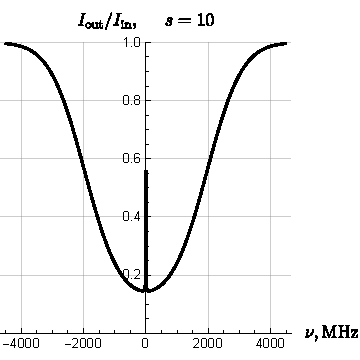
\includegraphics[width=0.33\textwidth]{"D:\\Kami\\git_folder\\notes_5sem\\rqc\\saturation_spectr_simulation\\frac2.pdf"}
    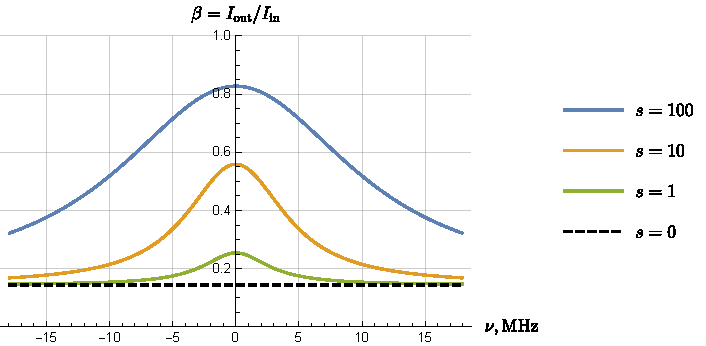
\includegraphics[width=0.63\textwidth]{"D:\\Kami\\git_folder\\notes_5sem\\rqc\\saturation_spectr_simulation\\frac1.pdf"}
    \caption{Спектр вблизи $\nu_{\text{рез}}$ при температуре в $300\ {}^{\circ}$С}
    \label{fig:frac12}
\end{figure}